\pdfoutput=1

\documentclass{article}

\usepackage[preprint]{tmlr}

\usepackage{amsmath,amssymb,amsthm}
\usepackage{booktabs}
\usepackage{multirow}
\usepackage{graphicx}
\usepackage{subcaption}
\usepackage{hyperref}
\usepackage{xcolor}
\usepackage{enumitem}
\usepackage{microtype}
\usepackage{array}
\usepackage[title]{appendix}

\newcommand{\NUM}[1]{\textbf{#1}}

\title{A Distributed Circuit in GPT-2 Found from Weights
and Missed by Activation-Based Discovery}

\author{\name Elliot Tower \\
      \email elliot@elliottower.ai}

\begin{document}

\maketitle

\begin{abstract}
Circuit discovery in mechanistic interpretability scores components by
individual causal effects on activations. When a circuit distributes
computation across many heads, every member falls below the
marginal-effect threshold individually, yet the ensemble mediates the
full causal effect. We report a 15-head circuit in GPT-2 Small whose
eight-head distributed tier is unrecoverable by five tested
activation-based methods---ACDC recovers 3 of 15 heads; activation
patching 1; EAP, EAP-IG, and copy scores recover zero---because
individual heads contribute near-zero while interactions account for
63\% of the total causal effect.

The circuit was assembled from weight matrices: $W_{OV}$ heatmaps
identify heads whose positive diagonals indicate token-copying capacity,
and K-composition scores ($\|W_O^{(i)} W_K^{(j)}\|_F$) trace inter-head
information flow. Composition analysis groups the 15 heads into four
tiers---three early-layer backbone heads, a midlayer detector, eight
mid-layer copier heads, and three readout heads. The circuit implements
Repeated Token Identification (RTI): copier heads attend preferentially
to non-repeated tokens and boost their logits, preventing the model
from regenerating content that has already appeared.

Weight-based and activation-based methods identify non-overlapping
circuit components (Jaccard $= 0.00$ at all tested scales).
The circuit outperforms ACDC's 30-head set at half the size. Ablating
it raises the repetition-degeneration rate from 0\% to 81\%
(Appendix~\ref{app:fragility}), yet its operating point is fragile:
perturbation in either direction disrupts generation equally.
\end{abstract}


%% =========================================================
\section{Introduction}
\label{sec:intro}
%% =========================================================

Circuit discovery in mechanistic interpretability follows a standard
workflow: run thousands of forward passes, record activations, patch
components, and infer structure from marginal effects
\citep{conmy2023acdc, goldowsky-dill2023localizing, syed2023eap}.
This approach has produced detailed accounts of several circuits---indirect
object identification \citep{wang2023ioi}, induction \citep{olsson2022icl},
greater-than comparison \citep{hanna2023gt}---and defines the field's
methodology.

We describe a circuit found by a different route. Rather than running
the model, we visualized its weight matrices as heatmaps
(Figure~\ref{fig:heatmap_example}) and identified heads sharing
geometric fingerprints (Figure~\ref{fig:l9h3_comparison}). Examining
144 pairs of $W_{OV}$ and $W_{QK}$ images, we traced visual
resemblances to a functional hypothesis: a cohort of heads with
positive-diagonal $W_{OV}$ matrices copies attended tokens into the
output logits, boosting non-repeated tokens.

The resulting circuit---15 heads organized into four tiers---handles
Repeated Token Identification (RTI) in GPT-2 Small. The RTI task was
designed \emph{after} the weight inspection, to test the hypothesis
that the visually similar heads promote non-repeated tokens.
The discovery sequence inverts the standard workflow: visual
observation $\to$ mechanistic hypothesis $\to$ task design $\to$
circuit assembly $\to$ causal validation, rather than the usual
task $\to$ activation analysis $\to$ circuit.

This inversion exposes a structural limitation of activation-based
methods. When a circuit tier distributes its computation across eight
heads, each contributing less than 5\% individually while 63\% of
the full effect arises from interactions, every marginal-effect method
drops the entire tier below threshold. Weight inspection identifies heads by
geometric similarity rather than marginal causal contribution, so it
does not depend on individual effect size.

The contribution is empirical: a novel distributed circuit, validated
by 19 causal experiments, whose largest tier no tested activation-based
method recovers (0/8 copier heads across five methods). The broader finding is that weight geometry and activation
analysis identify genuinely non-overlapping circuit components
(Jaccard $= 0.00$ across GPT-2 Small, Medium, Large, and XL).
Combining both perspectives outperforms either alone. We do not claim visual
inspection is a general-purpose discovery method; the automated
weight-feature classifier used for cross-model transfer
(\S\ref{sec:validation}) demonstrates that the same features scale
without human inspection.


%% =========================================================
\section{Weight Matrices as Heatmaps}
\label{sec:heatmaps}
%% =========================================================

Each attention head in a transformer has four weight matrices: $W_Q$,
$W_K$, $W_V$, $W_O$. The composite matrices $W_{OV} = W_V W_O$ and
$W_{QK} = W_Q^T W_K$ summarize the head's function: $W_{OV}$
determines what the head writes to the residual stream given an input,
and $W_{QK}$ determines what the head attends to
\citep{elhage2021mathematical}.

To make these matrices interpretable, we project them into token space:
the logit-level heatmap $W_E[:k] \cdot W_V W_O \cdot W_U[:, :k]$ has
entry $(i, j)$ equal to the contribution to token~$i$'s logit when the
head attends to token~$j$. We use $k = 50$ (the 50 most frequent
tokens); results are stable across
$k \in \{50, 100, 500, 1000\}$ (Spearman $\rho > 0.93$, all copier
heads maintain positive diagonal scores at every $k$).
We computed these heatmaps for all 144 attention heads in GPT-2
Small (12 layers $\times$ 12 heads) and arranged the resulting 288
images in a grid grouped by known circuit roles from prior work.

Three visual signatures correlate reliably with function:

\paragraph{Vertical banding in $W_{OV}$.}
Strong vertical stripes indicate that certain output dimensions are
activated regardless of input. A head whose $W_{OV}$ has prominent
vertical bars writes a fixed directional signal into the residual stream.
This pattern characterizes Layer~0 backbone heads that broadcast context
information through low-rank OV matrices (effective rank 33--37,
versus 57--62 for typical heads).

\paragraph{Diagonal structure.}
A dominant diagonal in $W_{OV}$ indicates copying: the head maps each
input dimension approximately to the same output dimension. Positive
diagonals (red in our color scheme) indicate token promotion; negative
diagonals (blue) indicate suppression. Heads with positive $W_{OV}$ diagonals and vertical banding---indicating
token-copying capacity---became the central observation of this study.

\paragraph{Uniform $W_{QK}$.}
Heads whose $W_{QK}$ matrices are nearly uniform (flat color, no
salient structure) attend broadly rather than selectively. These
tend to be positional or BOS-attending infrastructure heads, in
contrast to content-selective heads whose $W_{QK}$ matrices show
prominent diagonal or block structure.

\begin{figure}[t]
\centering
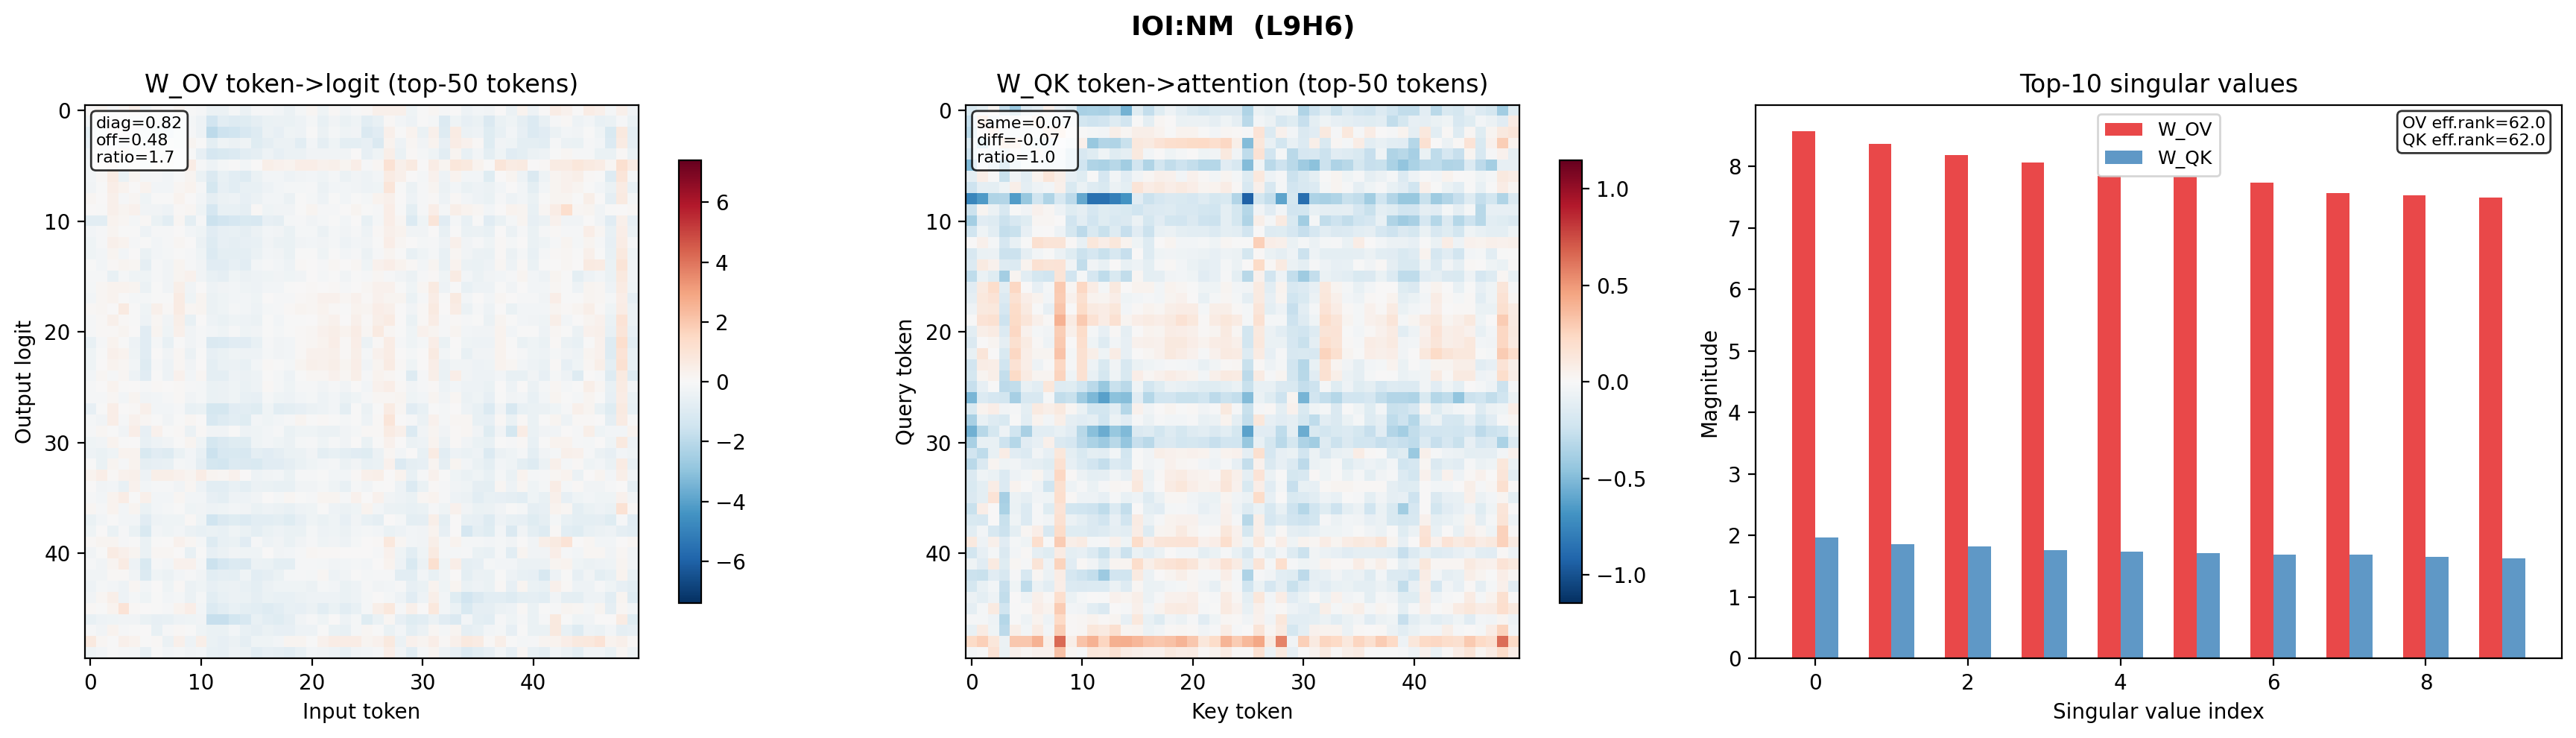
\includegraphics[width=\textwidth]{../figures/part1_role_heatmaps/heatmap_IOI_NM.png}
\caption{Weight fingerprint of an IOI Name Mover (L9H6). \textbf{Left:}
  $W_{OV}$ heatmap showing a positive diagonal (red, copying mode) with
  diag/off ratio $= 0.82$. \textbf{Center:} $W_{QK}$ showing content-selective
  attention (block structure, same/diff $= 0.07$). \textbf{Right:} Top-10
  singular values of $W_{OV}$ (red) and $W_{QK}$ (blue); effective rank
  62 for both indicates full-rank, content-dependent computation.
  The mid-layer heads that seeded this study show the opposite
  $W_{OV}$ signature: positive diagonal with vertical banding,
  indicating token-copying capacity.}
\label{fig:heatmap_example}
\end{figure}


%% =========================================================
\section{Discovery Process}
\label{sec:discovery}
%% =========================================================

The circuit was identified through four phases of progressively
focused visual analysis, all on a laptop CPU. No forward passes were
computed until the circuit hypothesis was fully assembled.

\subsection{Phase 1: Role Fingerprinting}

We computed weight-space features (SVD spectra, effective rank, $W_{OV}$
diagonal ratios, $W_{QK}$ same/different-token scores) for all 144 heads
and visualized them as heatmaps grouped by previously identified circuit
roles \citep{wang2023ioi, olsson2022icl}. Heads in the same circuit
role have visually similar weight fingerprints: name movers share one
pattern, S-inhibition heads share another, induction heads share a
third. Weight geometry encodes functional specialization, at least for
known circuits.

\subsection{Phase 2: Clustering}

A $t$-SNE embedding of all 144 heads by weight features confirmed the
visual impression (Figure~\ref{fig:tsne}): known circuit heads cluster
together, and several uncategorized heads fall near known roles. A
comparison panel placed each head next to its nearest known-circuit
neighbor, identifying which uncharacterized heads resemble which
circuit roles.

L9H3 appeared in the induction comparison panel as a ``random contrast''
head, but showed unexpected structure: strong $W_{OV}$ diagonal
(copying mode), negative $W_{QK}$ same/different ratio
(anti-induction), and a dominant SVD component.

\begin{figure}[t]
\centering
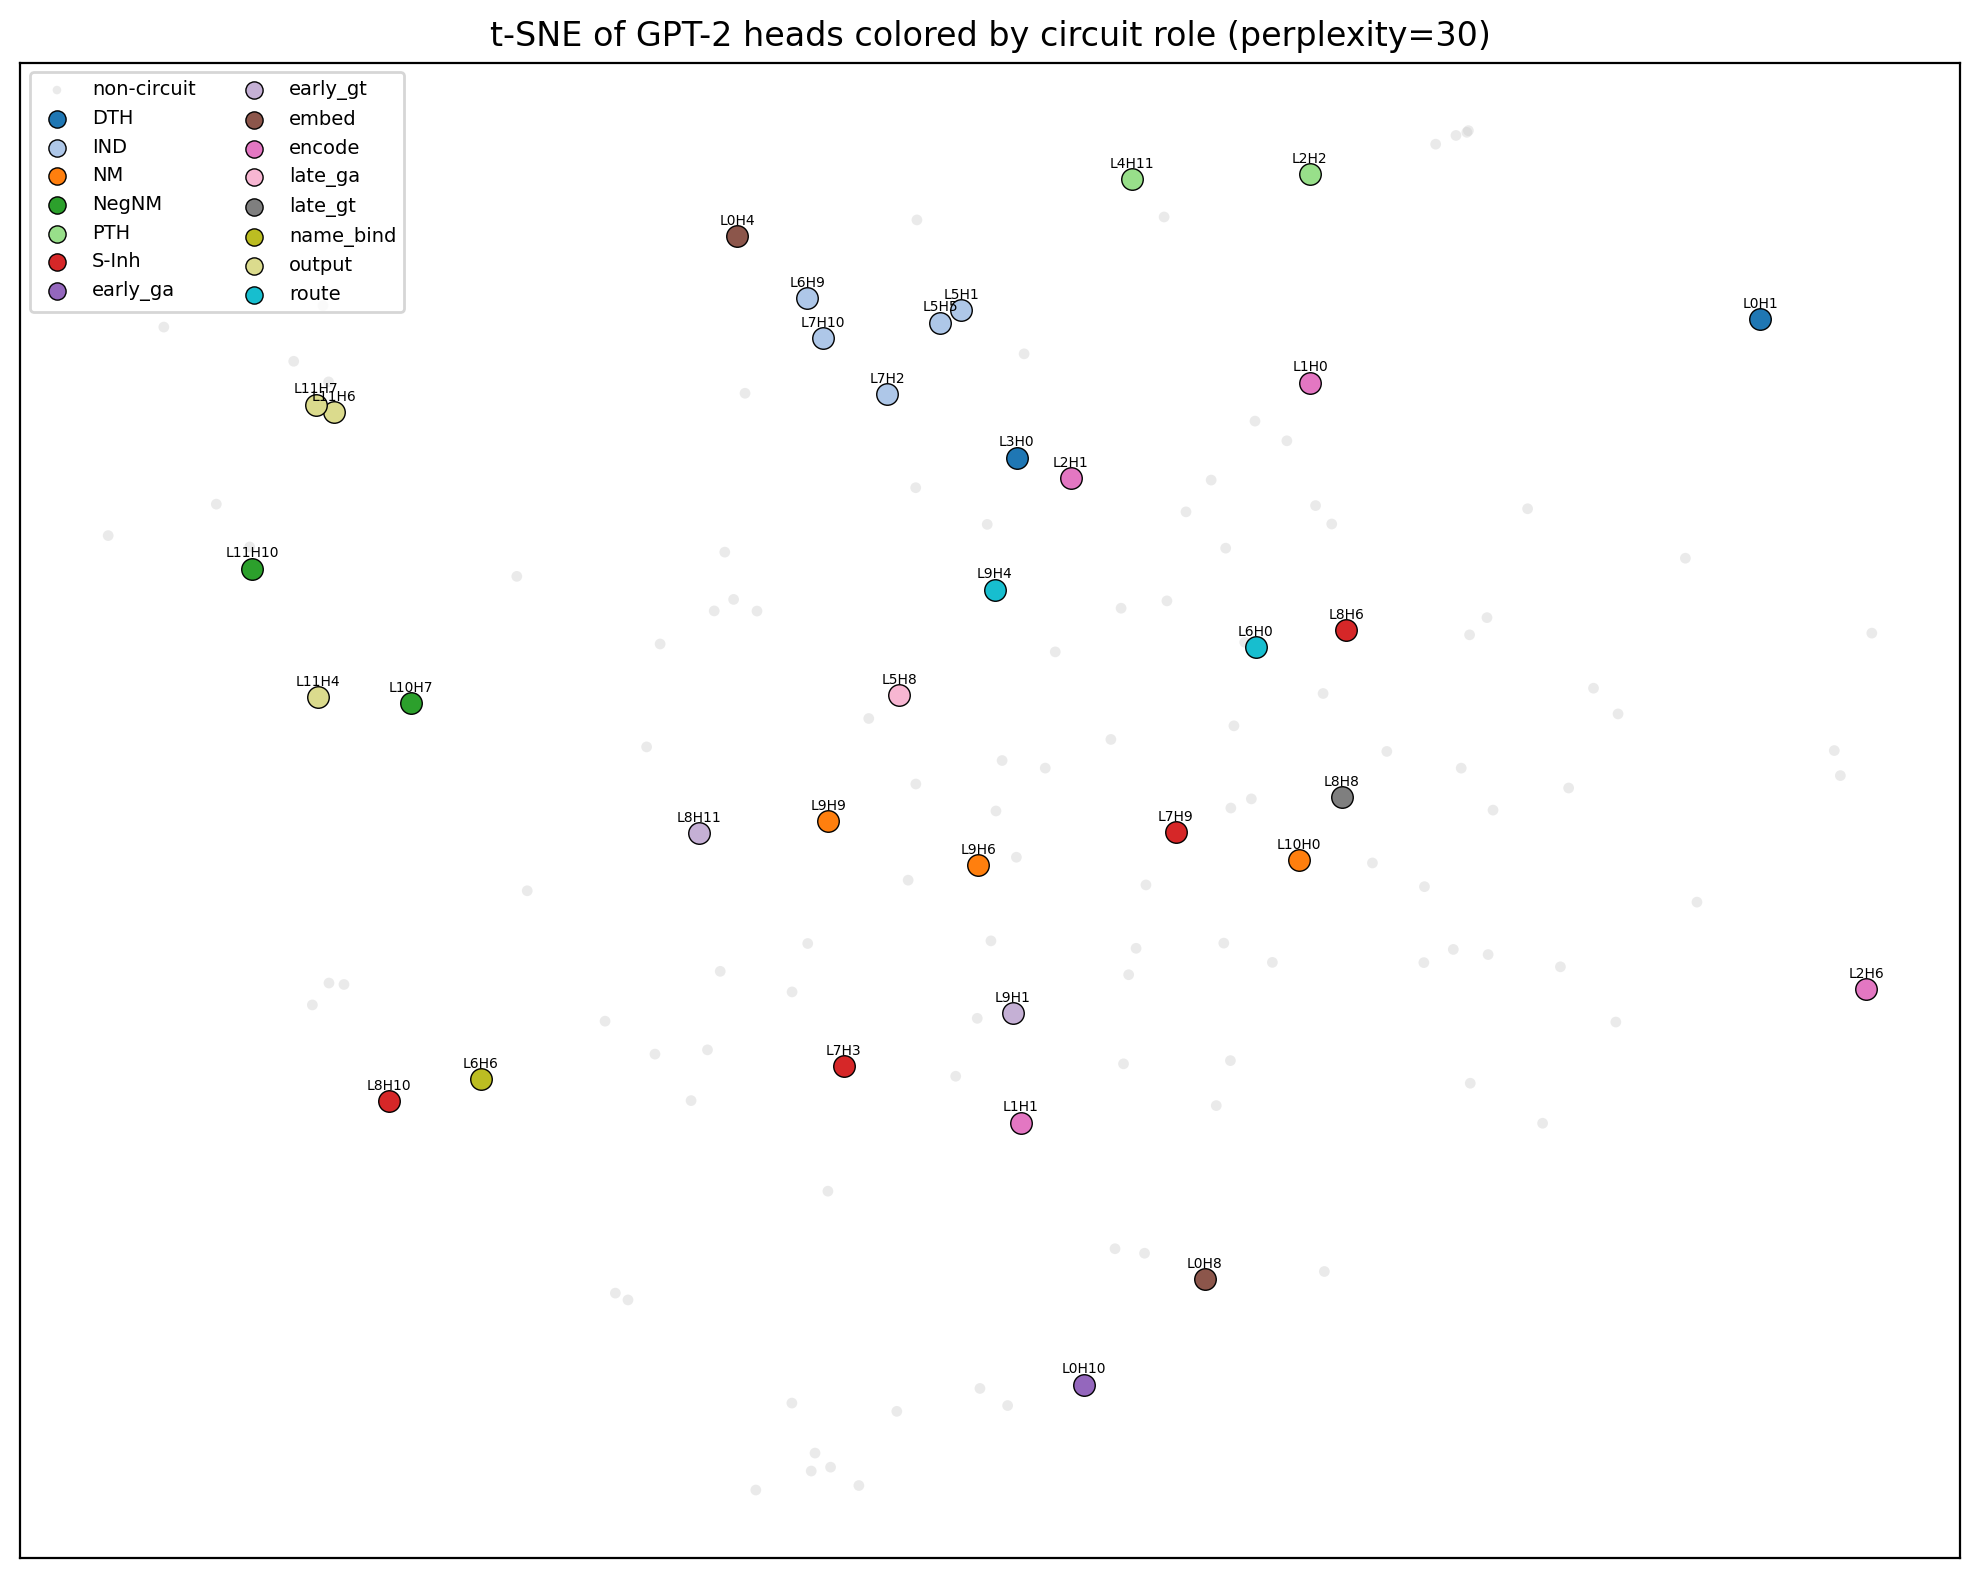
\includegraphics[width=0.85\textwidth]{../figures/part2_clustering/tsne_roles_annotated.png}
\caption{$t$-SNE of all 144 GPT-2 Small attention heads in weight feature
  space (perplexity~30), colored by known circuit role. Heads in the same
  functional role cluster together: name movers (orange), S-inhibition
  (red), induction (light blue), previous token heads (green). Gray dots
  are heads with no previously identified circuit role. The clustering
  confirms that weight geometry encodes functional specialization and
  provides the basis for identifying new circuit members by proximity
  to known roles.}
\label{fig:tsne}
\end{figure}

\subsection{Phase 3: The L9H3 Observation}

Examining Layer~8 and Layer~9 heatmaps in detail, two features of L9H3
stood out. First, its $W_{OV}$ consisted almost entirely of vertical
banding overlaid with a positive diagonal---the mirror image of
S-Inhibition heads, which show negative diagonals. Second, L9H10 was
visually near-identical (Figure~\ref{fig:l9h3_comparison}).

\begin{figure}[t]
\centering
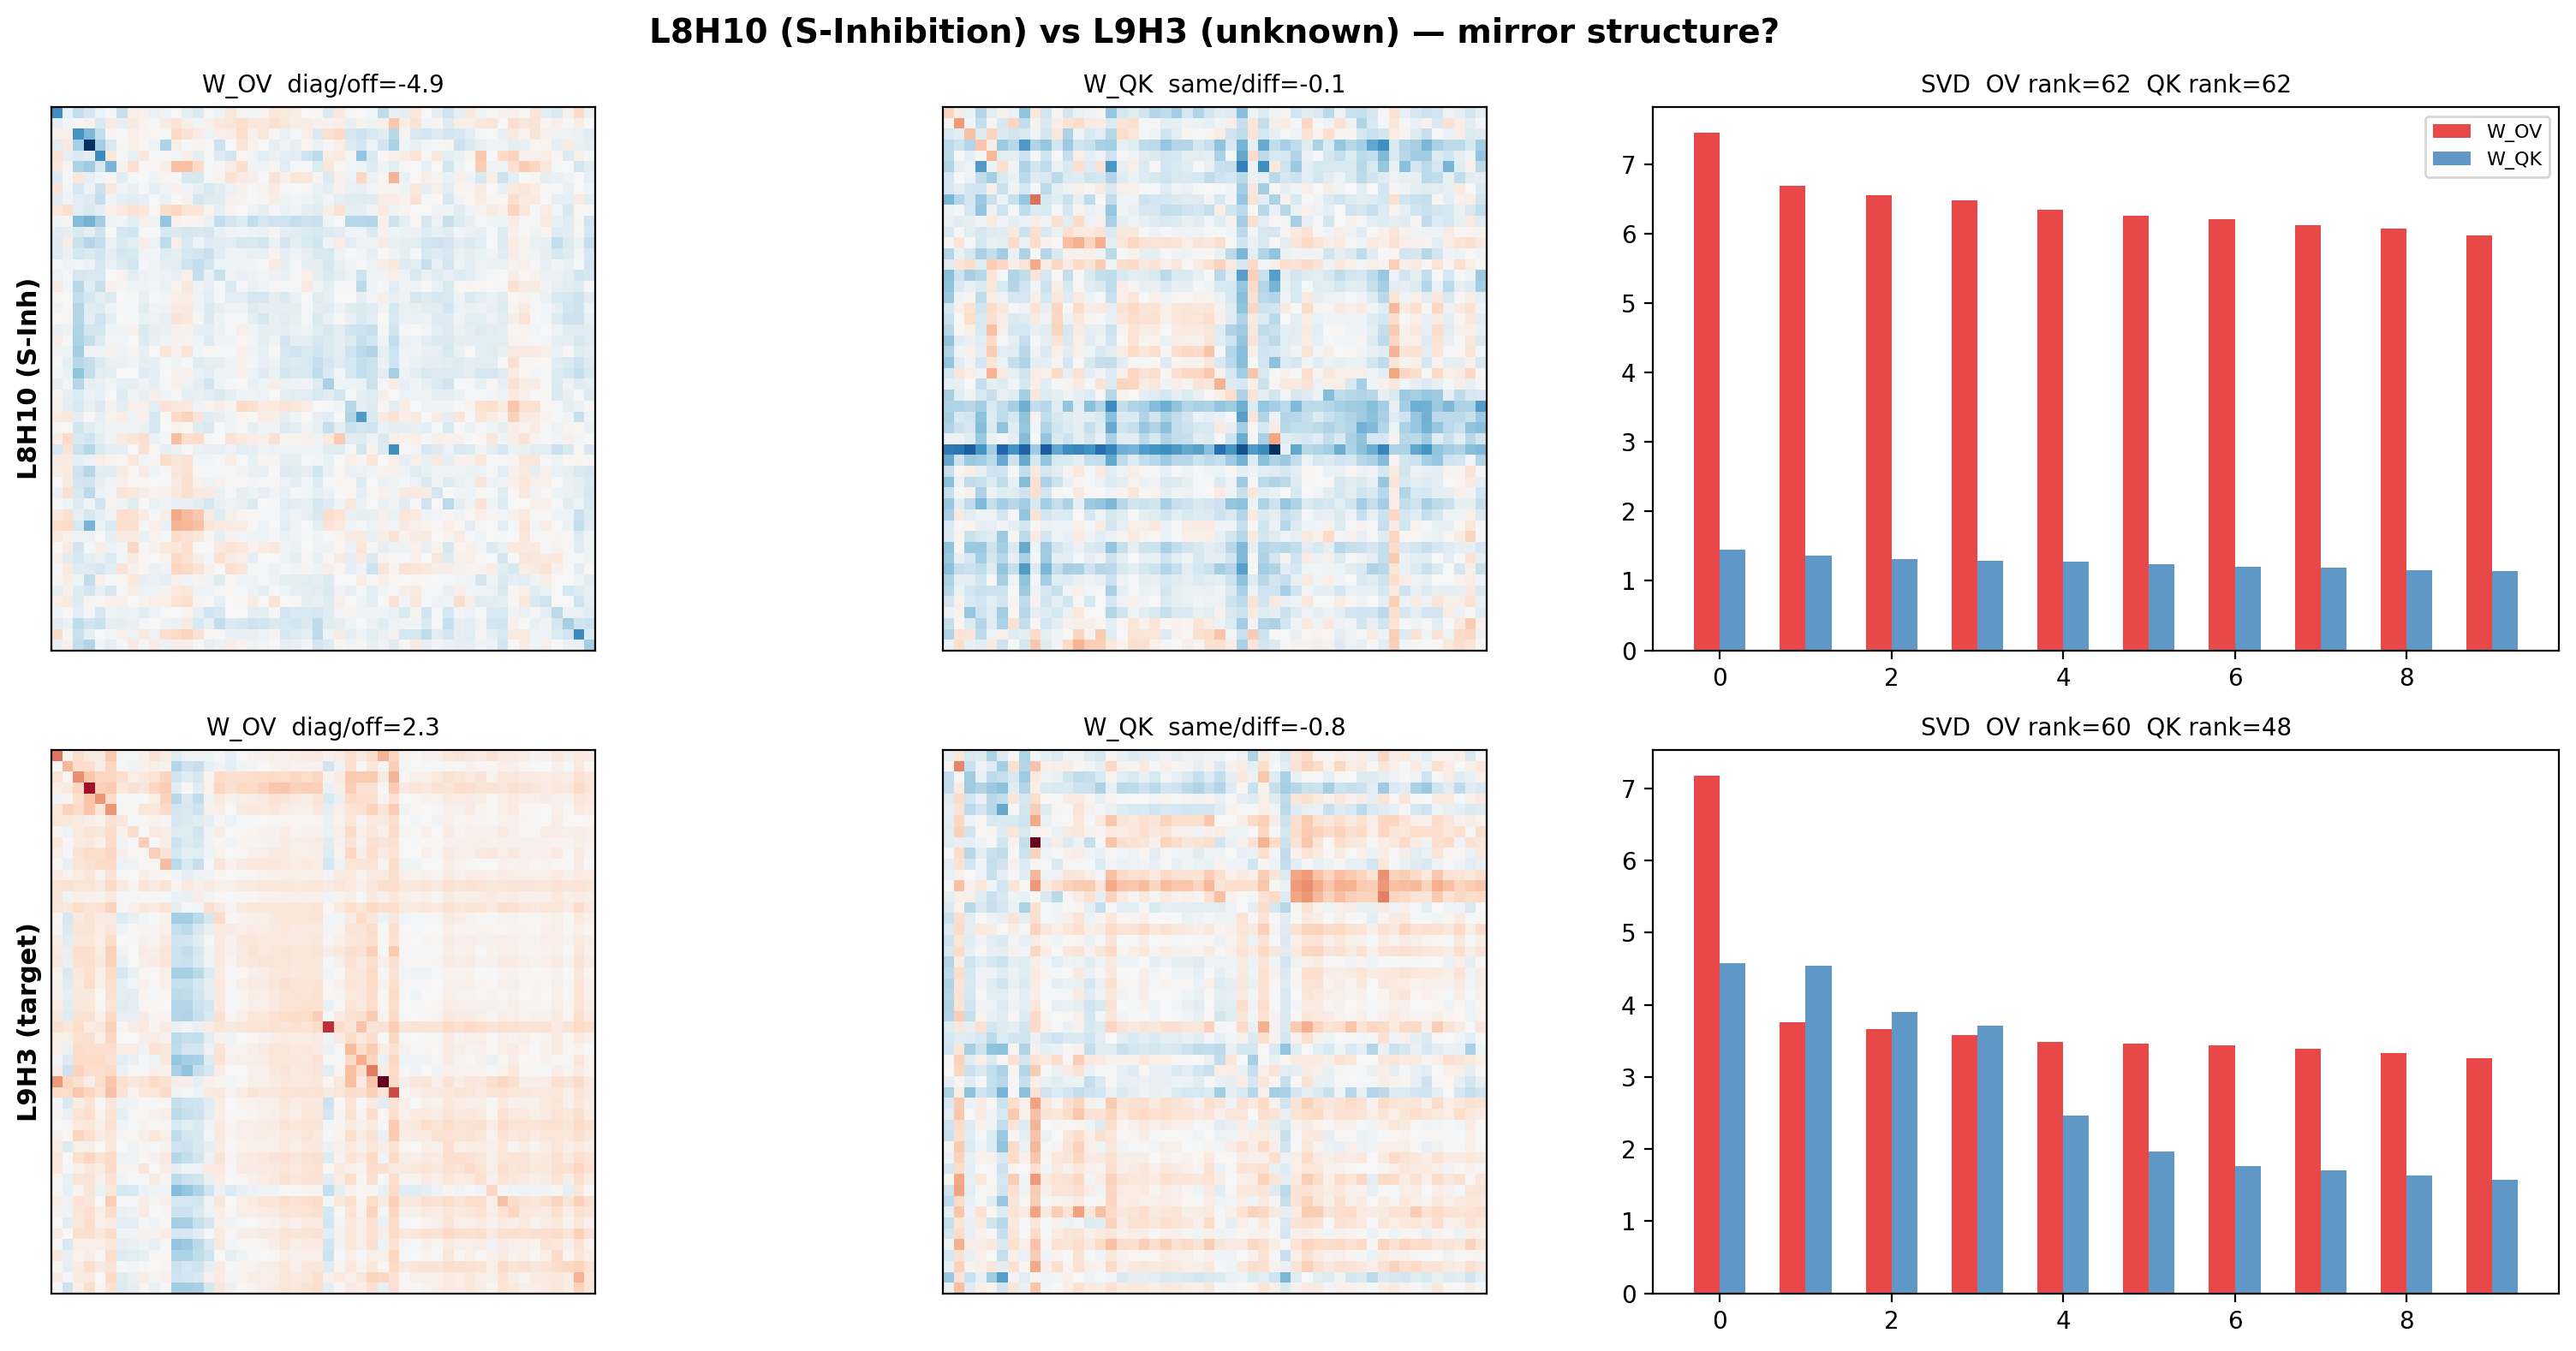
\includegraphics[width=\textwidth]{../figures/part3_l9h3/l8h10_vs_l9h3.png}
\caption{Weight fingerprints of L8H10 (S-Inhibition, known role) and L9H3
  (unknown, the investigation target). Each row shows $W_{OV}$
  (left), $W_{QK}$ (center), and SVD spectrum (right). L8H10 has a
  negative $W_{OV}$ diagonal (blue, diag/off $= -4.9$) characteristic
  of S-Inhibition heads. L9H3 shows the opposite: a positive diagonal
  (diag/off $= 2.3$) with vertical banding, a dominant first SVD
  component (7.1 versus 3.8 for the second), and a lower QK effective
  rank (48 versus 62). This ``mirror structure'' comparison---positive
  diagonal where S-Inhibition has negative---prompted investigation
  into L9H3's function.}
\label{fig:l9h3_comparison}
\end{figure}

This twin pair shared its visual signature---positive $W_{OV}$ diagonal
with vertical banding---with six other mid-layer heads: L4H0, L5H6,
L5H7, L7H0, L8H4, and L8H7.

The positive diagonal indicated a specific function: copy the logit
for whatever token the head attends to. A head that attends to
non-repeated tokens and boosts their logits would help the model
surface less-obvious correct completions over repeated alternatives.

\subsection{Phase 4: Hypothesis and Circuit Assembly}

The copying hypothesis predicted a specific functional role:
boost non-repeated tokens so the model can surface less-obvious
correct completions over repeated alternatives. This generated two
immediate consequences.

First, a new evaluation task. We designed Repeated Token Identification
(RTI): prompts where the correct completion is the \emph{non-repeated}
name (e.g., ``Then Alice and Bob went to the store. Alice gave a drink
to \underline{\phantom{Bob}}'' $\to$ Bob). If the mid-layer cohort
promotes non-repeated tokens, ablating it should impair RTI performance.

Second, a circuit hypothesis assembled from K-composition scores
(how strongly one head's output feeds another's key channel, measured
as $\|W_O^{(i)} W_K^{(j)}\|_F$;
background mean $= 10.4$, P95 $= 21.0$ across all head pairs).
Starting from L9H3 and L9H10---the two visually identified copier
heads---we traced composition edges in both directions. Downstream,
L10H11, L11H9, and L11H11 had the highest shared composition scores.
Upstream, three Layer~0 heads (L0H8, L0H9, L0H11) compose massively
with a midlayer relay (L4H11), with K-composition scores 76--130
versus 30--51 for non-circuit Layer~0 heads to the same target---a
$2$--$3\times$ gap above the P95 background level. Six additional
mid-layer heads (L4H0, L5H6, L5H7, L7H0, L8H4, L8H7) share both the
visual signature and the backbone's composition profile. Four heads
from the original visual cohort (L1H11, L3H10, L4H7, L11H5) share the
$W_{OV}$ pattern but have composition scores near background
(7--15, within P95), and were excluded.

The assembled circuit:
\begin{center}
\begin{tabular}{lll}
\toprule
\textbf{Tier} & \textbf{Heads} & \textbf{Count} \\
\midrule
Backbone & L0H8, L0H9, L0H11 & 3 \\
Detector & L4H11 & 1 \\
Copier & L4H0, L5H6, L5H7, L7H0, L8H4, L8H7, L9H3, L9H10 & 8 \\
Readout & L10H11, L11H9, L11H11 & 3 \\
\bottomrule
\end{tabular}
\end{center}

The entire assembly ran on a laptop CPU in approximately twelve hours.

\paragraph{Transparency note.}
The RTI task was designed \emph{after} the circuit hypothesis---to test
it, not to discover it. Had RTI failed to validate, a different task
could have been tried, and that failure would go unreported. Three
factors mitigate this concern: (i)~the circuit transfers without
modification to three independently defined tasks (SVA, IOI, gendered
pronoun; \S\ref{sec:validation}), (ii)~the composition-score filtering
applies a quantitative threshold (scores above background P95) rather
than post-hoc judgment, and (iii)~the visual discovery process,
including dead ends, is documented in the repository's lab notebooks.


%% =========================================================
\section{The RTI Circuit}
\label{sec:circuit}
%% =========================================================

The 15-head circuit implements a four-tier hierarchy for detecting and
completing repeated token sequences (Figure~\ref{fig:circuit_diagram}).
Each tier has a distinct weight signature and functional role.

\begin{figure}[t]
\centering
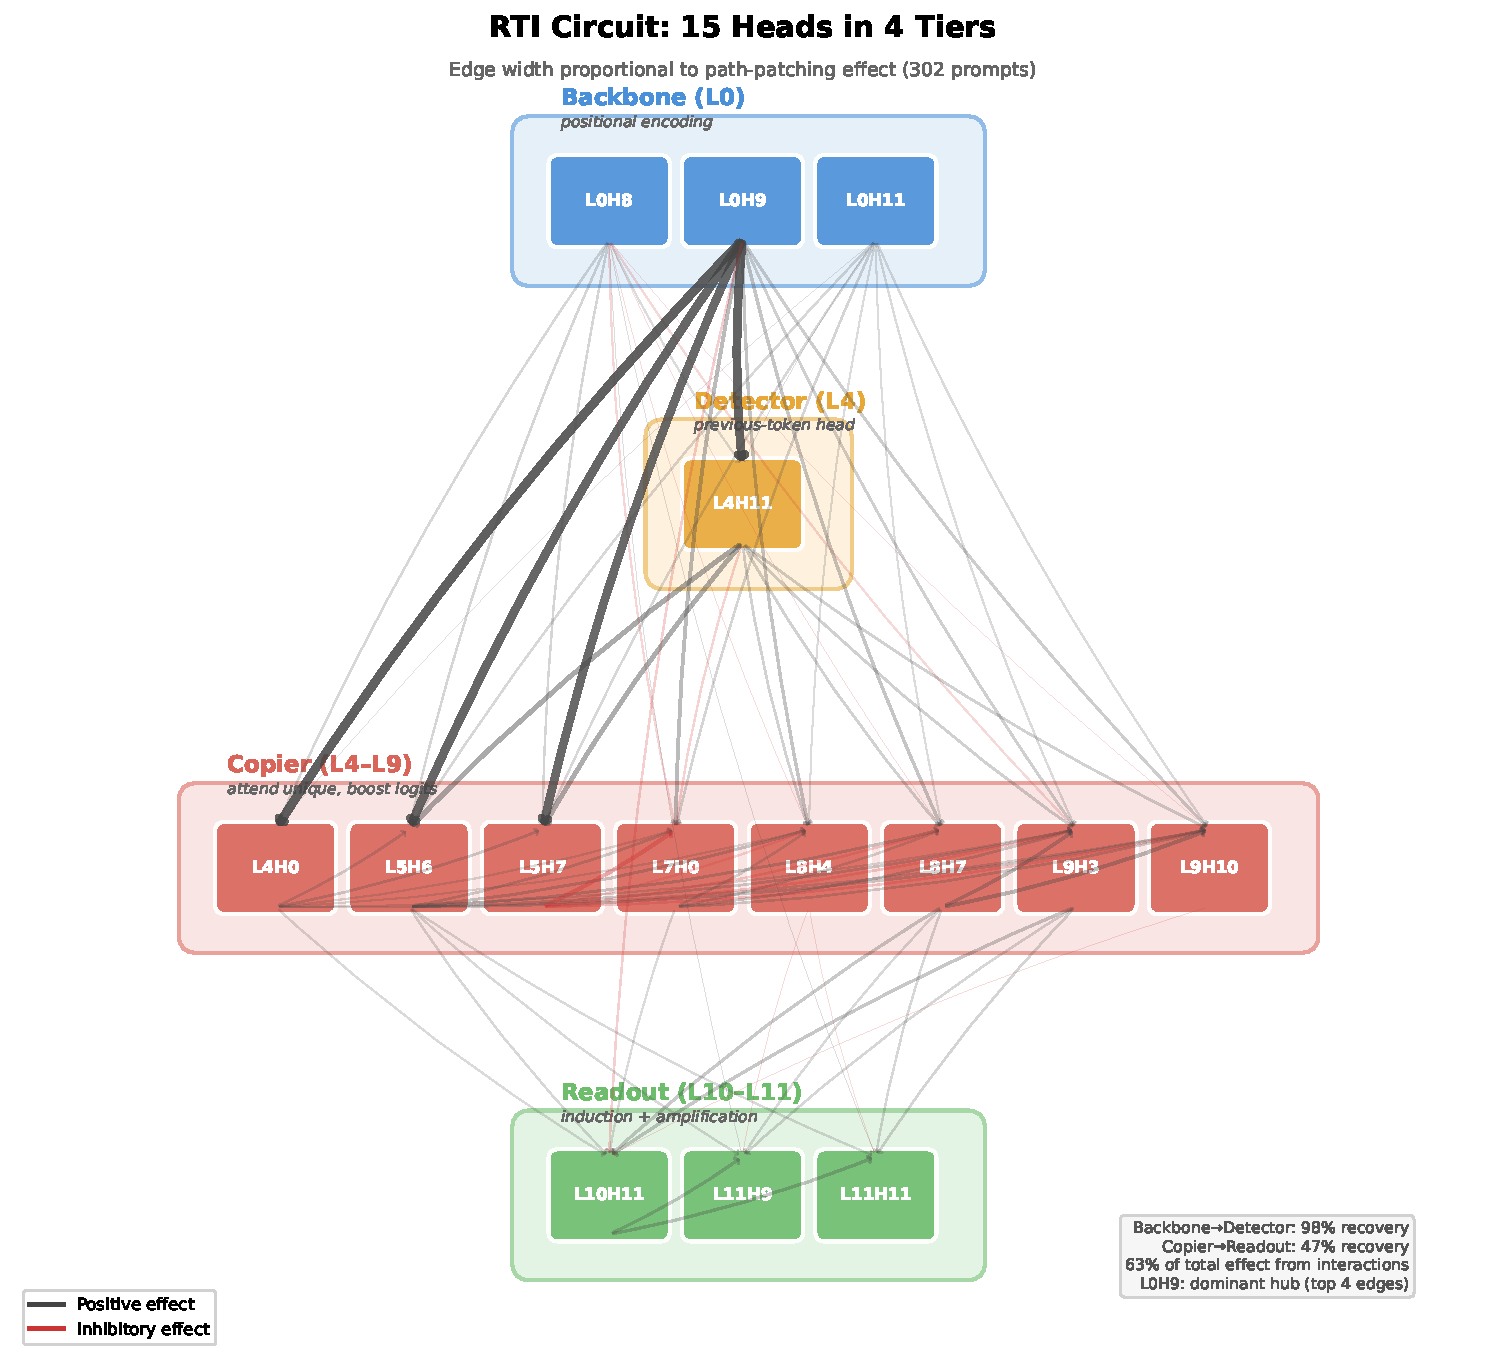
\includegraphics[width=0.85\textwidth]{generated_figures/rti_circuit_diagram.pdf}
\caption{The RTI circuit. Fifteen heads organized in four tiers;
  edge width is proportional to path-patching effect size (302 prompts).
  L0H9 is the dominant hub: its four strongest edges target L4H0,
  L4H11, L5H6, and L5H7 (each $0.16$--$0.17$ LD). The backbone
  $\to$ detector pathway carries 98\% of the full circuit effect.
  One inhibitory edge (L5H7 $\to$ L7H0, red) was detected.}
\label{fig:circuit_diagram}
\end{figure}

\subsection{Backbone (L0H8, L0H9, L0H11)}
\label{sec:backbone}

Three Layer~0 heads write fixed directional information into the
residual stream. Their OV effective rank (33--37) is the lowest in the
entire model (typical: 57--62), meaning their output concentrates in a
few singular vectors regardless of input content. They attend broadly
to context tokens (55--65\% attention to earlier context, versus 57--63\%
to the current token for non-circuit Layer~0 heads).

These heads produce the largest causal effect: zero-ablating all three
shifts the logit difference by $\Delta = -1.009$ (95\% CI
$[-1.332, -0.695]$, $n = 302$), accounting for 80\% of the full
circuit's effect ($\Delta = -1.267$).

L0H11 has the highest fan-out in the circuit---K-composition scores of
25--130 to every downstream target---yet the smallest individual
leave-one-out effect ($-0.402$). L0H9 has narrower fan-out but the
largest individual effect ($-0.439$). The explanation mirrors the
Backup Name Mover phenomenon in the IOI circuit \citep{wang2023ioi}:
L0H11's signal is replicated across redundant paths, so removing it
triggers backups. L0H9 carries a unique channel with no backup.

\subsection{Detector (L4H11)}

L4H11 is the critical relay between backbone and copiers. Its defining
property is an anomalous QK matrix: Frobenius norm 58.16, roughly
3--4$\times$ larger than any other head in the model. This massive QK
circuit reads the specific subspace directions that Layer~0 heads write,
enabling sharp detection of repeated positions (RTI attention fraction
0.303 on RTI prompts, rank 4/144 model-wide; attention entropy
0.018---near a delta function).

L4H11 is \emph{not} an induction head. Its prefix matching score is
$7.37 \times 10^{-23}$ (rank 144/144). Weight inspection
identified it as a backbone relay: K-composition scores from backbone
to L4H11 are 76--130, versus 30--51 for non-circuit Layer~0 heads to
the same target. This 2--3$\times$ gap is the weight-space signature
of the backbone-detector information channel.

L4H11 is GPT-2's previous token head---the same head classified as
a PTH in the IOI circuit \citep{wang2023ioi}. Weight inspection
identified it as a backbone relay from its K-composition profile;
follow-up experiments revealed its PTH identity. On 22 controlled
prompts where position $t{-}1$ and the repeated token occupy different
positions, L4H11 attended to $t{-}1$ in 15/18 valid tests. A
scaled confirmation (240 prompts from 12 templates $\times$
24 names, repeated token and $t{-}1$ always at different positions)
produced 240/240 PTH behavior: mean attention to $t{-}1 = 0.999$,
mean attention to repeated positions $= 0.000$. L2H2 (a known PTH)
showed 86\% PTH as a positive control; L11H9 (an induction head)
showed 0\% PTH as a negative control.

The circuit exploits a positional regularity of natural-language
repetition: in standard RTI prompts, the repeated token sits at
position $t{-}1$. The mechanism is ``attend backward then copy,''
not ``detect repetition then copy.''

L4H11 is the circuit's single bottleneck. Its 10 outgoing path-patching
edges sum to 97\% of the full circuit effect (302 prompts); 6 of 10
have 95\% CIs excluding zero, with the strongest pair targeting the
early copiers L5H6 and L5H7 ($0.074$ and $0.070$ LD each). The three
readout-targeted edges (L4H11 $\to$ L10H11, L11H9, L11H11) are near
zero, confirming that L4H11 communicates to readout through the copier
tier rather than directly.

\subsection{Copier Tier (8 Heads, L4--L9)}

The copier tier has no precedent in previously described circuits.
Standard induction circuits attend to a match and copy in the same head.
The RTI circuit splits these functions: the detector attends, and eight
distributed copier heads amplify. We call them ``copiers'' because their
$W_{OV}$ matrices have positive diagonals---the weight-space signature
of token copying---even though their activation-based copy scores are
near zero (0.03--0.59 versus 8--13 for readout heads;
Appendix~\ref{app:behavioral}). The name reflects structural capacity,
not activation-level behavior: these heads \emph{can} copy (the weights
encode it) but act indirectly through the residual stream rather than
through direct token-level copying. This gap between weight-space
capacity and activation-level behavior is the core of why activation
methods miss this tier.

Copier heads attend preferentially to non-repeated tokens, with
attention fractions to repeated positions ranging from 0.009 to 0.086
(Appendix~\ref{app:behavioral}). Most attend heavily to the BOS
position (56--82\% of attention mass), reading the accumulated residual
stream signal that contains the backbone's context encoding.
Eigenvalue copying scores increase with layer depth (9.4 at L4 to
171.4 at L9; full values in Appendix~\ref{app:behavioral}), consistent
with progressive amplification of the backbone signal.

Copiers are task-specific. L9H3's direct logit attribution across
other tasks is negligible: IOI ($+0.178$, rank 47/144), SVA
($+0.065$, rank 37/144), gendered pronoun ($-0.012$, rank 127/144).
These heads are RTI specialists with no role elsewhere.

No single copier is essential. Leave-one-out marginals range from
$-0.693$ (L9H10) to $+0.039$ (L5H7). Path patching shows the
copier $\to$ readout pathway recovers 47\% of the full circuit effect
(95\% CI $[24\%, 72\%]$). Exhaustive testing of
all $2^8 = 256$ copier subsets confirms that the best 4-copier subset
(\{L5H6, L5H7, L7H0, L9H3\}) slightly outperforms the full 8-copier
set---the extra copiers add mild interference, paralleling the
antagonistic readout finding described below.

The backbone heads write directional information into the residual
stream at Layer~0. By the time copiers at Layers~5--9 execute, this
information has accumulated at the BOS position (which every head can
attend to). Copiers read BOS to access the backbone's context signal;
the BOS token itself is irrelevant.

\subsection{Readout (L10H11, L11H9, L11H11)}

Two of the three readout heads are classic induction heads: L11H9
(prefix matching 0.322, copying 13.19) and L10H11 (prefix matching
0.295, copying 8.05). They do standard $[A][B] \ldots [A] \to B$
pattern matching and copy the next token.

L11H11 is different: low prefix matching (0.025) but anomalously low OV
rank (40.3) with a dominant top singular value (62.3, versus 18.6 for
L11H9). It writes in one specific direction with enormous magnitude---a
specialized amplification channel rather than a general-purpose induction
head. Its OV copy fraction (0.686) is the highest in the circuit.


%% =========================================================
\section{Causal Validation}
\label{sec:validation}
%% =========================================================

We validate the weight-derived circuit with 19 causal experiments
totaling approximately 40 GPU-hours. All experiments use the canonical
15-head circuit assembled from visual inspection
(Figure~\ref{fig:causal_validation}).

\begin{figure}[t]
\centering
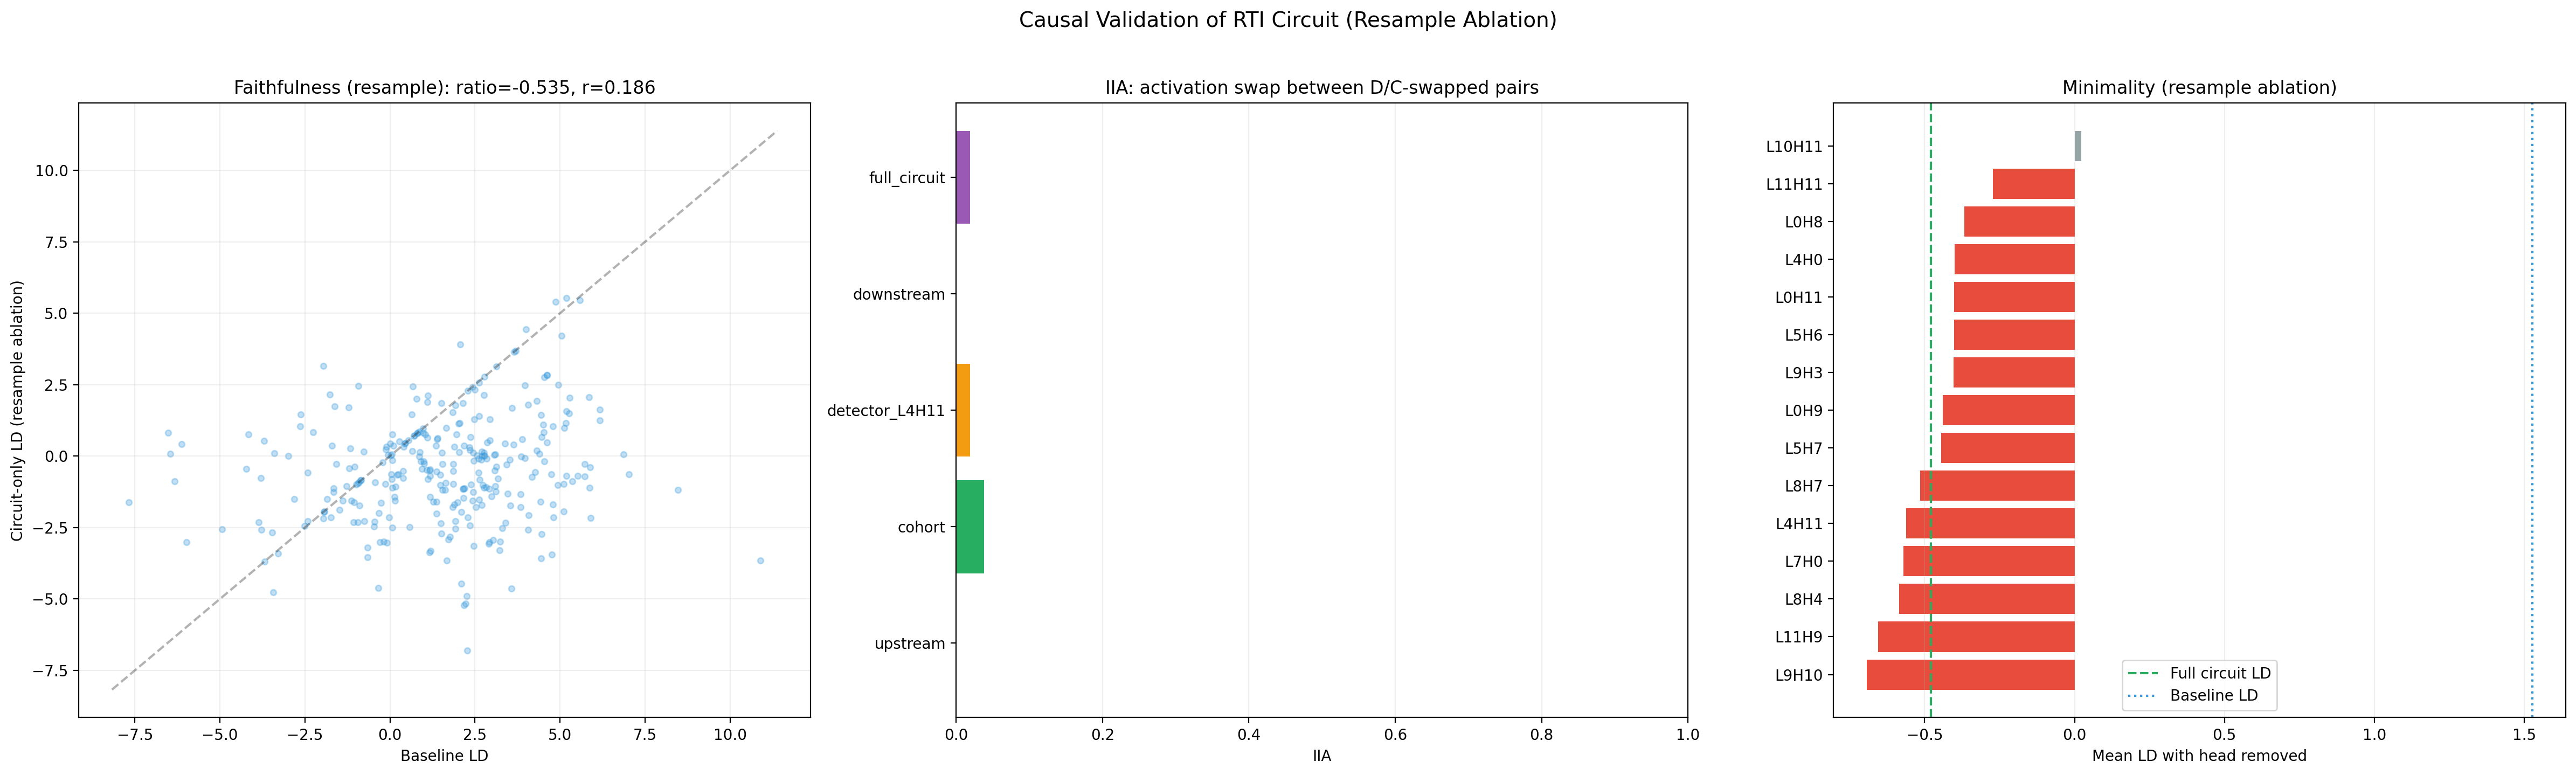
\includegraphics[width=\textwidth]{../figures/part4_causal_validation/causal_tests.png}
\caption{Causal validation of the weight circuit (resample ablation).
  \textbf{Left:} Faithfulness scatter---circuit-only logit difference
  versus baseline logit difference on 302 prompts ($r = 0.156$,
  95\% CI $[0.038, 0.269]$). The low correlation reflects prompt-level
  variance: the circuit is necessary (ablation destroys performance)
  but the per-prompt logit difference depends on factors outside
  the 15-head circuit. \textbf{Center:} IIA (interchange intervention
  accuracy) by tier. The full circuit achieves IIA comparable to
  the detector alone; the copier cohort shows a large effect while
  upstream heads are tightly localized.
  \textbf{Right:} Minimality (leave-one-out resample ablation) for all
  15 heads. All heads except L10H11 have negative LOO effect (removing
  them hurts), confirming minimality. L10H11's redundancy mirrors the
  Backup Name Mover phenomenon \citep{wang2023ioi}.}
\label{fig:causal_validation}
\end{figure}

\subsection{Ablation}

On 302 RTI prompt pairs (baseline mean LD $= 1.526$, 95\% CI
$[1.227, 1.834]$), full circuit zero-ablation shifts the mean logit
difference by $\Delta = -1.267$ (95\% CI $[-1.651, -0.888]$,
$p = 0.032$, permutation test). Resample ablation (replace circuit head
activations with activations from random other inputs) gives a
completeness drop of $-0.511$ (95\% CI $[-0.655, -0.370]$).
Per-prompt faithfulness correlation is modest ($r = 0.156$), comparable
to partial circuits in other work---a 15-head subset of a 144-head
model is necessary for the task but does not account for all
prompt-level variance in logit difference.

The effect decomposes hierarchically. The Layer~0 trio alone produces
$\Delta = -1.009$ (95\% CI $[-1.332, -0.695]$). The copier cohort
alone gives $\Delta = -0.117$ (95\% CI $[-0.218, -0.019]$, $n = 302$).
The downstream readout alone gives $\Delta = +0.039$ (95\% CI
$[-0.001, +0.078]$) under zero ablation---a positive shift.
Multi-method ablation resolves this paradox: under resample ablation,
removing any readout head \emph{hurts} performance
(L10H11: $-0.023$ $[-0.045, -0.002]$;
L11H9: $-0.023$ $[-0.042, -0.004]$;
L11H11: $-0.003$ $[-0.025, +0.017]$).
The ``antagonism'' is a zero-ablation artifact: zeroing a head's
output is more disruptive than replacing it with plausible
activations, and the circuit compensates for the disruption.

\textbf{Interaction effects.}
The 15 individual leave-one-out marginals sum to only $-0.461$---36\%
of the full circuit effect ($-1.267$). The remaining 63\% (95\% CI
$[49\%, 76\%]$) arises from interactions between heads. Decomposing
further: tier-level ablations sum to $-0.986$ (78\% of the full
effect), so within-tier interactions account for ${\sim}41\%$ and
cross-tier interactions for ${\sim}22\%$. The copier tier contributes
most of the within-tier interaction---individual copiers have marginals
near zero (four are positive, meaning removal helps), yet the tier
collectively amplifies the backbone signal. This interaction structure
explains why marginal-effect methods miss the copier tier entirely.

\subsection{Path Patching}

Edge-level path patching \citep{wang2023ioi} on all 97 intra-circuit
edges (302 prompts) traces information flow through the circuit
(Table~\ref{tab:path}). Each edge is isolated by patching the sender
head from a corrupted input, freezing all intermediate attention heads
to clean activations, and letting only the receiver head recompute;
post-receiver layers recompute normally. Pathway recoveries measure
overlapping causal chains---backbone $\to$ detector captures 98\%
because corruption at this bottleneck propagates through all downstream
tiers.

\begin{table}[h]
\centering
\caption{Path patching recovery by pathway (ratio-of-means,
302 prompts, bootstrap 95\% CI). Full circuit effect: 0.235 LD.
Pathways measure overlapping causal chains, so recoveries do not
sum to 100\%.}
\label{tab:path}
\begin{tabular}{lcc}
\toprule
\textbf{Pathway} & \textbf{Recovery} & \textbf{95\% CI} \\
\midrule
Backbone $\to$ detector & 98.3\% & $[68.7, 128.3]$ \\
Copier $\to$ readout & 47.1\% & $[23.6, 71.7]$ \\
Backbone $\to$ copier & 16.6\% & $[0.9, 32.6]$ \\
Detector $\to$ copier & 11.1\% & $[3.5, 19.0]$ \\
Backbone $\to$ readout & 3.2\% & $[-3.6, 10.1]$ \\
Detector $\to$ readout & 0.1\% & $[-4.8, 5.0]$ \\
\bottomrule
\end{tabular}
\end{table}

The backbone $\to$ detector pathway dominates (98.3\%), confirming
that L4H11 is a single bottleneck through which backbone information
must pass. This is consistent with the K-composition gap analysis
(\S\ref{sec:backbone}): backbone $\to$ detector has a clean gap of
$+19.4$ between circuit and non-circuit edges, while other pathways
show no separation. The copier $\to$ readout pathway carries 47\%,
with the remaining pathways near or below the noise floor.

L0H9 is the critical hub: the four strongest individual edges are all
L0H9 $\to$ \{L4H0, L4H11, L5H6, L5H7\}, each with effect $0.16$--$0.17$
(95\% CIs excluding zero). One inhibitory edge was detected:
L5H7 $\to$ L7H0 $= -0.054$ ($[-0.081, -0.029]$), consistent with
L5H7's positive leave-one-out marginal (removing it helps).

\subsection{Localization}

\textbf{DAS.}
Distributed Alignment Search \citep{geiger2024das} localizes the causal
variable to Layers~10--11 (Table~\ref{tab:das}). DAS finds where the
variable is \emph{represented} in the residual stream, not where
it is \emph{computed}---the backbone and detector heads compute at
L0 and L4, but their output accumulates into a representation that
becomes interventable only at later layers. The variable is
partially formed at Layer~8 (IIA plateaus at 0.79 even at $k = 64$)
and fully crystallized by Layer~10 (IIA $= 1.00$ at $k = 16$). Random
IIA is zero everywhere.

\begin{table}[h]
\centering
\caption{DAS IIA by layer and subspace dimensionality $k$.}
\label{tab:das}
\begin{tabular}{lcccccc}
\toprule
\textbf{Layer} & $k{=}1$ & $k{=}4$ & $k{=}8$ & $k{=}16$ & $k{=}32$ & $k{=}64$ \\
\midrule
L0--L4 & 0 & 0 & 0 & 0 & 0 & 0 \\
L6 & 0.01 & 0.02 & 0.01 & 0.01 & 0.04 & 0.04 \\
L8 & 0.12 & 0.48 & 0.67 & 0.74 & 0.78 & 0.79 \\
L10 & 0.21 & 0.76 & 0.96 & \NUM{1.00} & \NUM{1.00} & \NUM{1.00} \\
L11 & 0.23 & 0.80 & \NUM{1.00} & \NUM{1.00} & \NUM{1.00} & \NUM{1.00} \\
\bottomrule
\end{tabular}
\end{table}

\textbf{Logit lens} \citep{nostalgebraist2020logitlens}\textbf{.}
A sharp phase transition occurs at Layer~9: logit
difference jumps to $+5.712$ with per-layer attribution of $+34.6$.
Layer~11 actively suppresses ($-13.1$), paralleling the IOI Negative
Name Mover pattern \citep{wang2023ioi}. The DAS result matches: the
causal variable becomes fully interventable one layer after the logit
lens signal appears.

\textbf{Probes.}
A linear probe trained to detect ``this token has appeared before''
reaches 84\% accuracy at Layer~0 and 100\% by Layer~2, with
cross-set generalization gap of $-0.3\%$ (trained on names A--H,
tested on I--P). The model represents repetition as an abstract
concept by Layer~2---well before the copier tier begins amplifying it.

\textbf{SAE attribution.}
SAE feature causal analysis concentrates in Layer~9: four of the five
most causally important features (effects 0.63--0.71) reside in Layer~9.
Per-layer maximum effects follow the circuit topology:
L0 (0.12) $\to$ L4 (0.33) $\to$ L7 (0.65) $\to$ L9 (0.71). These
features are pre-existing SAE directions with no learned alignment to
the task, sidestepping the representation alignment concern raised by
\citet{sutter2025alignment}.

\subsection{Cross-Task Transfer}

The weight circuit, identified on RTI, transfers to three other tasks
without modification:

\begin{itemize}[itemsep=2pt]
\item \textbf{SVA} (Subject-Verb Agreement \citep{lazo2025sva}): 12/12
  ground truth heads recovered, 3 false positives. Progressive ablation
  curves match ground truth.
\item \textbf{IOI} (Indirect Object Identification): 13/26 ground truth
  heads recovered, 4 false positives. Sufficiency: weight $= -0.022$
  versus GT $= -0.018$. Progressive ablation AUC: weight $= 0.600$
  versus random $= 0.214$ (3$\times$ better).
\item \textbf{Gendered Pronoun} \citep{mathwin2023gp}: 5/5 ground truth
  heads recovered.
\end{itemize}

The backbone and readout tiers transfer across all tasks; the detector
and copier tiers are task-specific. L6H0 serves as the SVA analogue of
L4H11's detector role.

\subsection{Cross-Model Transfer}

The weight circuit transfers zero-shot across the GPT-2 model family.
We extract the same 108 spectral weight features for every head in
GPT-2 Medium (24 layers, 384 heads) and Large (36 layers, 720 heads),
apply the bootstrap classifier trained on Small's ground truth labels,
and measure IIA at varying confidence thresholds
(Table~\ref{tab:cross_model}).

\begin{table}[h]
\centering
\caption{IIA at varying bootstrap stability thresholds on GPT-2 Large.
  The transition from IIA\,=\,1.0 to IIA\,=\,0.0 occurs over a narrow
  threshold range, revealing that low-confidence heads are causally
  critical.}
\label{tab:cross_model}
\begin{tabular}{rcccccc}
\toprule
\textbf{Threshold} & \textbf{IOI $|C|$} & \textbf{IOI IIA} &
  \textbf{SVA $|C|$} & \textbf{SVA IIA} &
  \textbf{GT $|C|$} & \textbf{GT IIA} \\
\midrule
0.0 & 214 (30\%) & \NUM{1.000} & 205 (28\%) & \NUM{0.917} & 106 (15\%) & \NUM{1.000} \\
0.1 & 111 (15\%) & \NUM{1.000} & 100 (14\%) & \NUM{0.917} & 57 (8\%) & \NUM{1.000} \\
0.3 & 53 (7\%) & 0.212 & 34 (5\%) & 0.000 & 24 (3\%) & \NUM{0.939} \\
0.7 & 5 (0.7\%) & 0.000 & 7 (1\%) & 0.000 & 5 (0.7\%) & \NUM{0.909} \\
\bottomrule
\end{tabular}
\end{table}

On GPT-2 Large, swapping all 20 heads at Layer~0 alone achieves
IIA\,=\,1.0 for IOI and Greater-Than, with logit shifts of 8.46 and
3.16. No other single layer achieves IIA\,$> 0.5$ for any task. These
20 heads constitute 2.8\% of the 720 total.

This bottleneck is absent on GPT-2 Medium, where no single layer
achieves IIA\,$> 0.5$. Greedy head addition on Large IOI reveals the
mechanism: eight late-layer heads (L18--L32) accumulate logit shift from
0.134 to 1.453 with IIA fixed at zero; five Layer-0 heads then produce
a discontinuous jump (L0H3 alone contributes $+0.651$ IIA). The late-layer
heads build task-relevant information that requires Layer-0's initial
positional encoding to become causally sufficient.

Weight-predicted and EAP/EAP-IG circuits show 0--1/15 overlap at
Medium, Large, and XL (Table~\ref{tab:overlap_scale}). The disjointness
observed on Small generalizes: weight features and edge attribution
identify genuinely different head populations at every tested scale.
Combining them (weight $t{=}0.5$ + EAP top-15) achieves IIA\,=\,1.0
on all three tasks on Medium, outperforming either method alone.

\begin{table}[h]
\centering
\caption{Overlap between weight circuit and EAP-IG top-15 across
  scales. Near-zero overlap persists at every scale.}
\label{tab:overlap_scale}
\small
\begin{tabular}{llcc}
\toprule
\textbf{Scale} & \textbf{Task} & $|$\textbf{WC}$|$ & \textbf{EAP-IG $\cap$ WC} \\
\midrule
Medium & IOI & 13 & 1/15 \\
       & SVA & 5 & 0/15 \\
Large  & IOI & 5 & 0/15 \\
       & SVA & 7 & 0/15 \\
XL     & IOI & 10 & 1/15 \\
       & SVA & 8 & 0/15 \\
\bottomrule
\end{tabular}
\end{table}


%% =========================================================
\section{Comparison with Automated Discovery Methods}
\label{sec:comparison}
%% =========================================================

We compared the visual weight circuit against five automated discovery
methods on the RTI task (Table~\ref{tab:methods}). Each method selected
its top 15 heads (ACDC selects 30 by its own criterion).

This comparison is asymmetric by design: the weight circuit was
assembled through iterative human analysis, while each automated
method ran a single pass. The comparison tests whether each method's
\emph{scoring criterion}---marginal causal effect, gradient
attribution, or greedy pruning---recovers the distributed tier, not
whether the methods are given equal compute budgets. The key question
is structural: can any marginal-effect threshold recover a tier
where every member contributes $<5\%$ individually? The answer is no,
regardless of compute budget, because the scoring criterion itself
discards distributed components.

\begin{table}[h]
\centering
\caption{Causal validation of each method's selected heads on an
expanded 200-prompt RTI set (baseline mean LD: $+2.243$; this set
predates the 302-prompt set used in \S\ref{sec:validation}). Zero and
resample ablation of each method's head set. The weight circuit is the
only set whose ablation flips the sign of the logit difference.}
\label{tab:methods}
\begin{tabular}{lccccc}
\toprule
\textbf{Method} & \textbf{Heads} & \textbf{Zero $\Delta$} & \textbf{Resample $\Delta$} & \textbf{Flips LD?} & \textbf{Zero/Resample} \\
\midrule
\textbf{Weight (visual)} & 15 & $-2.464$ & $-0.355$ & Yes & 6.94 \\
EAP & 15 & $-1.566$ & $-1.711$ & No & 0.91 \\
EAP-IG & 15 & $-1.731$ & $-1.932$ & No & 0.90 \\
ActPatch & 15 & $-1.067$ & $-1.372$ & No & 0.78 \\
ACDC & 30 & $-1.942$ & $-1.029$ & No & 1.89 \\
\bottomrule
\end{tabular}
\end{table}

\subsection{Zero versus resample ablation}

Table~\ref{tab:methods} also reports the ratio of zero-ablation to
resample-ablation effect (rightmost column). For the weight circuit,
zero ablation is 6.94$\times$ worse than resample ablation: replacing
circuit head outputs with zeros destroys the computation entirely, but
replacing them with outputs from other RTI prompts partially preserves
the copying behavior. For EAP and EAP-IG, the ratio is approximately
0.9---zeros and random replacements produce nearly identical effects.

This asymmetry distinguishes task-specific computation from
general-purpose importance. The weight circuit heads perform a specific
function (promoting non-repeated tokens) that zero ablation destroys but
resample ablation partially preserves. EAP's heads contribute general
language modeling capacity that any perturbation disrupts equally.

\subsection{Per-Tier Recovery by Method}

Table~\ref{tab:tier_recovery} reveals why the methods disagree: each is
sensitive to a different aspect of circuit function.

\begin{table}[h]
\centering
\caption{Per-tier recall for each discovery method. Copy score
ranks heads by logit contribution to the repeated token
\citep{wang2023ioi}. The weight method is the only method that
recovers every tier.}
\label{tab:tier_recovery}
\begin{tabular}{lccccc}
\toprule
\textbf{Tier} & \textbf{Weight} & \textbf{EAP/EAP-IG} & \textbf{ActPatch} & \textbf{ACDC} & \textbf{Copy score} \\
\midrule
Backbone (3) & \NUM{3/3} & 0/3 & 0/3 & 2/3 & 0/3 \\
Detector (1) & \NUM{1/1} & 0/1 & \NUM{1/1} & \NUM{1/1} & 0/1 \\
Copier (8)   & \NUM{8/8} & 0/8 & 0/8 & 0/8 & 0/8 \\
Readout (3)  & \NUM{3/3} & 0/3 & 0/3 & 0/3 & 2/3 \\
\midrule
Total (15)   & \NUM{15/15} & 0/15 & 1/15 & 3/15 & 2/15 \\
\bottomrule
\end{tabular}
\end{table}

The copier tier has zero overlap with all five automated methods
combined: eight heads, five methods, no intersection. Each copier
contributes less than 5\% individually (mean activation patching
effect $+0.015$), placing them below every marginal-effect threshold.

\subsection{Exact gradients}

If EAP's failure were due to gradient approximation, exact gradients
should fix it. We computed exact gradients for all 32,491 edges in GPT-2
Small---one forward pass per edge, 5.5 hours of GPU time. Top-15 recall:
0/15. The same two heads found by approximate EAP (L0H9, L11H11) appear
in the top~30. The weight method finds 14/15 in 2 minutes on CPU (the
missed head, L4H0, has the weakest composition scores in the copier
tier). The failure is structural: exact and approximate gradients
agree on what to rank highly, and neither ranks distributed
components.


%% =========================================================
\section{Weight Capacity versus Causal Flow}
\label{sec:capacity}
%% =========================================================

The clearest example of weight--activation alignment involves L0H9.
This head has the second-highest K-composition score to the detector
(111.2), the largest individual leave-one-out effect among backbone
heads ($-0.439$), and the strongest edge-level causal flow: the four
largest path-patching effects in the circuit are all L0H9 $\to$
\{L4H0, L4H11, L5H6, L5H7\}, each $0.16$--$0.17$ LD.

Weight analysis measures \emph{capacity}: the structural ability of one
head's output to influence another's computation, as encoded in the
geometry of $W_O^{(i)} W_K^{(j)}$. Edge-level path patching
measures \emph{flow}: the information actually transmitted on a given
input distribution. For L0H9, capacity and flow align---both identify
it as the circuit's dominant hub.

This pattern generalizes. K-composition scores between the copier tier
and readout tier are low (mean 10.3, near the random baseline of 7.6),
yet path patching shows the copier $\to$ readout pathway recovers
47\% of the circuit effect. The copiers communicate through
the residual stream rather than direct composition. Weight analysis
identifies structural connectivity; activation analysis identifies
which channels carry signal on a given distribution. A method that
captures only one perspective will miss components visible from the
other.


%% =========================================================
\section{Discussion}
\label{sec:discussion}
%% =========================================================

\subsection{Prerequisites for Visual Discovery}

The discovery required domain expertise in two areas. First, familiarity
with the mathematical framework for transformer circuits
\citep{elhage2021mathematical}, which guided interpretation of $W_{OV}$
and $W_{QK}$ structure. Second, knowledge of existing circuit taxonomies
(IOI, induction, S-inhibition), which provided reference patterns for
visual comparison. Without these reference points, the heatmaps would
have been uninterpretable noise.

The RTI task was designed \emph{after} the circuit hypothesis was formed,
inverting the usual circuit-explains-task direction: the task was chosen
to test a weight-derived hypothesis.

\subsection{The Distributed Copier Tier}

The copier tier's distributed structure is what weight inspection
recovers and activation methods miss. Standard induction heads attend to
a match and copy within a single head; the RTI circuit separates
detection from amplification across nine heads (one detector plus eight
copiers). No single copier exceeds 5\% individual contribution, yet 63\%
of the full causal effect arises from interactions among heads.

This architecture is unrecoverable by marginal-effect methods by
construction: each member is individually below threshold, so no
threshold setting recovers the tier without also selecting dozens of
false positives. Weight geometry identifies heads by shared
structure---two heads with identical $W_{OV}$ patterns (L9H3 and
L9H10) are recognized as functional twins regardless of their
individual causal importance.

\subsection{Limitations}

\paragraph{Scaling.}
The cross-model transfer results (\S\ref{sec:validation}) show that
the weight circuit generalizes within the GPT-2 family. Whether
\emph{visual} discovery scales is a separate question. GPT-2 Small has
288 heatmaps; a 96-layer, 96-head model produces 18,432. Automated
weight-feature classification can handle arbitrary scale, but the
visual inspection step that generated the initial hypothesis does not.

\paragraph{Subjectivity.}
The discovery involved judgment calls---which visual patterns to follow,
which heads to group together, how to design the confirmatory task.
Different investigators examining the same heatmaps would likely
reach different intermediate hypotheses. The final circuit is validated
by automated experiments, but the path to it is not reproducible in the
way an algorithm is.

\paragraph{Post-hoc risk.}
The RTI task was designed to test a weight-derived hypothesis, not
discovered independently. Had validation failed, a different task
could have been tried, creating a garden-of-forking-paths concern.
Three factors bound this risk: (i)~the circuit transfers without
modification to three independently defined tasks (SVA, IOI, gendered
pronoun), none of which were designed for it; (ii)~the composition-score
filtering uses a quantitative threshold (above P95 of all head-pair
scores) rather than subjective judgment; (iii)~the full discovery
process, including dead ends, is documented in the repository.

\paragraph{Threshold sensitivity.}
The heatmap computation uses the top $k = 50$ tokens by embedding
index; diagonal scores are stable across $k \in \{50, 100, 500, 1000\}$
(Spearman $\rho > 0.93$; all copier heads maintain positive scores at
every $k$). The backbone$\to$detector composition pathway has a gap of
19.4 between the weakest circuit edge (76.0) and the strongest
non-circuit edge (56.7). Other pathways (detector$\to$copier,
copier$\to$readout) have scores near the background mean and
communicate through the residual stream rather than direct composition.
All 15 circuit heads participate in at least one above-P95 edge;
at P99, 10/15 survive.

\paragraph{Statistical coverage.}
Bootstrap 95\% CIs ($n_{\text{boot}} = 10{,}000$) are reported for all
ablation effects, leave-one-out minimality values, and faithfulness
correlations ($n = 302$ prompts). Degeneration rates are averaged over
5 generation seeds per condition. Path-patching recovery fractions use ratio-of-means bootstrap
CIs (Table~\ref{tab:path}). Future work should vary prompt
sets and random seeds to bound estimator variance separately from
prompt-set variance.


%% =========================================================
\section{Related Work}
\label{sec:related}
%% =========================================================

Activation-based circuit discovery methods---ACDC
\citep{conmy2023acdc}, EAP \citep{syed2023eap}, activation
patching \citep{goldowsky-dill2023localizing}, DAS
\citep{geiger2024das}---all require forward passes and score components
by individual contributions. Distributed circuits where each member
falls below the marginal-effect threshold are unrecoverable by this
approach. \citet{marks2024sparse} find circuits at SAE feature
granularity rather than head granularity; whether feature-level
decomposition recovers distributed heads that head-level methods
miss is an open question.

Weight-space analysis has a longer history.
\citet{elhage2021mathematical} established that $W_{OV}$ and $W_{QK}$
encode head function and that composition scores measure inter-head
information flow. \citet{olsson2022icl} used composition scores to
identify induction heads. \citet{elhelo2025maps} and
\citet{golimblevskaia2025circuitlens} classify head function from
parameters. We extend these from individual head characterization to
full circuit discovery through systematic visual inspection. The IOI
circuit \citep{wang2023ioi} was identified through a semi-manual
process involving activation patching heatmaps; our process is
analogous but operates on weight matrices.

\citet{sutter2025alignment} showed that arbitrarily powerful alignment
maps can achieve 100\% IIA on randomly initialized models, making
DAS with non-linear maps vacuous. Weight-only analysis sits at the
opposite extreme: no learned alignment map, no risk of overfitting
to spurious activation correlations.

On cross-model comparison, \citet{olsson2022icl} studied induction
heads across scales but focused on behavioral properties, and
\citet{bhaskar2024consistent} scaled edge-based circuit discovery
to models 100$\times$ larger than prior methods. Our cross-model transfer adds
a specific finding: weight-space features identify a scale-dependent
Layer-0 bottleneck that is causally sufficient on Large but absent on
Medium.

On repetition degeneration, \citet{holtzman2020curious} documented the
phenomenon and proposed nucleus sampling. \citet{wang2025induction}
proposed log descaling of induction heads, but their method finds 0/15
RTI heads and makes degeneration worse. Our circuit provides a
mechanistic account of an anti-repetitive mechanism in GPT-2
(Appendix~\ref{app:fragility}).


%% =========================================================
\section{Conclusion}
\label{sec:conclusion}
%% =========================================================

We report a 15-head circuit in GPT-2 Small assembled entirely from
weight-matrix analysis: $W_{OV}$ heatmaps identified candidate heads
by functional signature, and K-composition scores traced their
connectivity. The circuit's eight-head copier tier---individually
below every marginal-effect threshold, with 63\% of the total causal
effect arising from interactions---is unrecoverable by all five tested
activation-based methods. The circuit prevents repetition
degeneration (0\% $\to$ 81\% on ablation; Appendix~\ref{app:fragility}),
but operates at a fragile equilibrium: amplification is as destructive
as ablation (U-shaped dose-response). The circuit transfers zero-shot to GPT-2 Medium and
Large, revealing a Layer-0 bottleneck where 2.8\% of heads achieve
perfect IIA on two benchmark tasks.

The broader finding is that weight-based and activation-based circuit
discovery identify non-overlapping components (Jaccard $= 0.00$ at
all tested scales). Distributed circuits are structurally invisible to
marginal-effect scoring, and weight geometry is structurally blind to
flow-dependent computation. Combining both perspectives outperforms
either alone.

\paragraph{Code and data availability.}
All analysis code, circuit definitions, causal validation scripts,
prompt sets, and raw experimental results are available at
\url{https://github.com/ElliottTower/rti-circuit}.
The 61 figures from the discovery process, including all heatmaps
and validation plots, are archived in the repository under
\texttt{c1\_manual\_investigation/figures/}.


%% =========================================================
\bibliographystyle{tmlr}
\bibliography{references}
%% =========================================================


%% =========================================================
\begin{appendices}

\section{Repetition Degeneration and Circuit Fragility}
\label{app:fragility}

If the RTI circuit promotes non-repeated tokens, ablating it should
cause the model to degenerate into repetition loops. This prediction
holds---but a second prediction, that amplifying the circuit should
reduce degeneration, fails. The circuit operates at a critical
point where perturbation in either direction is equally destructive.

\begin{center}
\begin{tabular}{lcc}
\toprule
\textbf{Condition} & \textbf{Degeneration rate} & \textbf{$\Delta$ from baseline} \\
\midrule
Baseline (full model) & $0 \pm 0$\% (5 seeds) & --- \\
Backbone ablation (3 heads) & $78.0 \pm 9.3$\% (5 seeds) & $+78.0$ pp \\
Full circuit ablation (15 heads) & $81.0 \pm 9.2$\% (5 seeds) & $+81.0$ pp \\
Random 15-head control & $0 \pm 0$\% (5 seeds) & $0$ pp \\
\bottomrule
\end{tabular}
\end{center}

The effect is concentrated in the backbone: ablating only three Layer~0
heads raises degeneration to $78.0 \pm 9.3$\%, nearly matching the full
15-head ablation ($81.0 \pm 9.2$\%). Neither the baseline nor the
pre-registered random 15-head control produces any degeneration across
5 generation seeds, confirming the effect is circuit-specific.

The circuit is anti-repetitive: it prevents degenerate loops.

If the circuit prevents repetition, amplifying it should decrease
degeneration. This prediction is wrong. Scaling backbone outputs by
$2\times$ raises degeneration to 75.9\% ($+28.4$ pp); at $3\times$,
to 90.3\% ($+42.8$ pp)---\emph{worse} than complete ablation. The
dose-response curve is U-shaped: both weakening and strengthening the
circuit disrupts generation. The safe perturbation zone spans
approximately $0.75$--$1.5\times$ the pretrained magnitude. The
circuit's output magnitude appears tightly coupled with downstream
expectations; perturbation in either direction disrupts the balance.

Six circuit-informed intervention strategies---detector gating,
single-head ablation, residual direction editing, entropy-gated scaling,
circuit-aware penalty, and contrastive decoding---all fail to reduce
degeneration. Circuit-based degeneration detectors (L4H11 attention
threshold, circuit logit ratio) perform at chance: the circuit activates
identically during legitimate and degenerate generation. Standard
repetition penalty ($p = 1.2$), which requires zero circuit knowledge,
fixes all 16 degenerate prompts with no quality loss.

The U-shaped dose-response curve suggests the circuit operates at a
learned equilibrium: its output magnitude is tightly calibrated to
downstream expectations, and any perturbation---whether ablation or
amplification---breaks this calibration. At least for this circuit,
identifying the mechanism did not yield a targeted intervention.


\section{Full Causal Validation Results}
\label{app:causal}

\subsection{Ablation Tests}

\begin{table}[h]
\centering
\begin{tabular}{llccc}
\toprule
\textbf{Test} & \textbf{Type} & \textbf{$\Delta$} & \textbf{95\% CI} & \textbf{$n$} \\
\midrule
Full circuit (15 heads) & Zero & $-1.267$ & $[-1.651, -0.888]$ & 302 \\
L0 trio only & Zero & $-1.009$ & $[-1.332, -0.695]$ & 302 \\
Detector only & Zero & $-0.045$ & $[-0.115, +0.016]$ & 302 \\
Copier cohort only & Zero & $-0.117$ & $[-0.218, -0.019]$ & 302 \\
Readout only & Zero & $+0.039$ & $[-0.001, +0.078]$ & 302 \\
Full circuit & Resample & $-0.511$ & $[-0.655, -0.370]$ & 302 \\
Pre-reg random 15 & Zero & $+0.149$ & $[-0.010, +0.305]$ & 302 \\
Other L0 (H0, H1, H3) & Zero & $-0.282$ & $[-0.350, -0.217]$ & 302 \\
Random 3 late & Zero & $+0.046$ & $[-0.016, +0.107]$ & 302 \\
\bottomrule
\end{tabular}
\end{table}

\subsection{Minimality (Resample Leave-One-Out)}

Resample ablation over 302 prompts with 95\% bootstrap CIs
($n_{\text{boot}} = 10{,}000$).

\begin{table}[h]
\centering
\begin{tabular}{llccc}
\toprule
\textbf{Rank} & \textbf{Head} & \textbf{Tier} & \textbf{LOO $\Delta$} & \textbf{95\% CI} \\
\midrule
1 & L4H11 & Detector & $-0.172$ & $[-0.270, -0.086]$ \\
2 & L0H9 & Backbone & $-0.076$ & $[-0.112, -0.041]$ \\
3 & L9H3 & Copier & $-0.075$ & $[-0.104, -0.047]$ \\
4 & L5H6 & Copier & $-0.064$ & $[-0.096, -0.034]$ \\
5 & L0H8 & Backbone & $-0.061$ & $[-0.092, -0.030]$ \\
6 & L8H7 & Copier & $-0.051$ & $[-0.075, -0.027]$ \\
7 & L7H0 & Copier & $-0.030$ & $[-0.050, -0.012]$ \\
8 & L11H9 & Readout & $-0.023$ & $[-0.042, -0.004]$ \\
9 & L10H11 & Readout & $-0.023$ & $[-0.045, -0.002]$ \\
10 & L0H11 & Backbone & $-0.005$ & $[-0.016, +0.007]$ \\
11 & L11H11 & Readout & $-0.003$ & $[-0.025, +0.017]$ \\
12 & L8H4 & Copier & $+0.005$ & $[-0.009, +0.018]$ \\
13 & L4H0 & Copier & $+0.014$ & $[-0.008, +0.038]$ \\
14 & L9H10 & Copier & $+0.022$ & $[+0.011, +0.034]$ \\
15 & L5H7 & Copier & $+0.081$ & $[+0.042, +0.125]$ \\
\bottomrule
\end{tabular}
\end{table}

Seven of 15 heads have CIs entirely below zero (removing them
significantly hurts the circuit). L4H11 has the largest individual
effect ($-0.172$). Five copier-tier heads have CIs overlapping zero,
consistent with high redundancy: no single copier is essential.
L5H7 is the only head whose removal \emph{helps} ($+0.081$,
CI excludes zero), suggesting mild interference at full capacity.

\subsection{Sufficiency Comparison}

\begin{table}[h]
\centering
\begin{tabular}{lccc}
\toprule
& \textbf{Weight (15)} & \textbf{Ground Truth (15)} & \textbf{ACDC (30)} \\
\midrule
Sufficiency (mean) & $-0.736$ & $-0.736$ & $-0.344$ \\
Sufficiency (resample) & $-1.024$ & $-1.023$ & $-0.021$ \\
Necessity FP & 2 & 0 & 27 \\
\bottomrule
\end{tabular}
\end{table}


\section{K-Composition Scores}
\label{app:kcomp}

Background statistics (all head pairs where sender layer $<$ receiver
layer): mean $= 10.44$, std $= 6.95$, P95 $= 21.04$.

\subsection{Backbone $\to$ Detector}

\begin{table}[h]
\centering
\begin{tabular}{lcc}
\toprule
\textbf{Sender} & \textbf{K-comp} & \textbf{Z-score} \\
\midrule
L0H11 $\to$ L4H11 & 130.4 & 17.2 \\
L0H9 $\to$ L4H11 & 111.2 & 14.5 \\
L0H8 $\to$ L4H11 & 76.0 & 9.4 \\
\midrule
L0H3 $\to$ L4H11 (control) & 50.6 & 5.8 \\
L0H1 $\to$ L4H11 (control) & 37.2 & 3.9 \\
L0H0 $\to$ L4H11 (control) & 30.1 & 2.8 \\
\bottomrule
\end{tabular}
\end{table}

\subsection{Pathway Summary}

\begin{table}[h]
\centering
\begin{tabular}{lcccc}
\toprule
\textbf{Pathway} & \textbf{Edges} & \textbf{Strong} & \textbf{Mean K-comp} & \textbf{Max K-comp} \\
\midrule
Backbone $\to$ detector & 3 & 3 & 105.9 & 130.4 \\
Backbone $\to$ copier & 24 & 22 & 36.2 & 55.5 \\
Backbone $\to$ readout & 9 & 9 & 27.1 & 42.3 \\
Detector $\to$ copier & 7 & 0 & 7.8 & 9.2 \\
Detector $\to$ readout & 3 & 0 & 6.4 & 7.1 \\
Copier $\to$ readout & 24 & 2 & 8.9 & 15.3 \\
\bottomrule
\end{tabular}
\end{table}

Two information transfer mechanisms: backbone $\to$ \{detector, copier\}
operates through K-composition (scores 27--130, far above background).
Detector $\to$ copier and copier $\to$ readout operate through the
residual stream (scores 6--9, near background).


\section{Behavioral Census}
\label{app:behavioral}

Full behavioral census on 500 general sequences for all 15 circuit
heads. RTI attention fractions are lower than on dedicated RTI prompts
(e.g., L4H11: 0.234 general vs.\ 0.303 on RTI prompts) because general
text contains fewer repeated-token positions.

\begin{table}[h]
\centering
\small
\begin{tabular}{llcccc}
\toprule
\textbf{Head} & \textbf{Tier} & \textbf{Prefix} & \textbf{Copy} & \textbf{RTI attn} & \textbf{BOS attn} \\
\midrule
L0H8  & Backbone & 0.017 & $-0.16$ & 0.025 & 0.073 \\
L0H9  & Backbone & 0.017 & $-0.28$ & 0.061 & 0.298 \\
L0H11 & Backbone & 0.022 & $-0.85$ & 0.066 & 0.309 \\
L4H11 & Detector & 0.000 & $+0.17$ & \NUM{0.234} & 0.000 \\
L4H0  & Copier   & 0.000 & $+0.04$ & 0.020 & 0.376 \\
L5H6  & Copier   & 0.000 & $+0.35$ & 0.086 & 0.694 \\
L5H7  & Copier   & 0.000 & $+0.10$ & 0.009 & 0.567 \\
L7H0  & Copier   & 0.000 & $+0.23$ & 0.078 & 0.567 \\
L8H4  & Copier   & 0.000 & $+0.03$ & 0.017 & 0.751 \\
L8H7  & Copier   & 0.000 & $+0.32$ & 0.030 & 0.592 \\
L9H3  & Copier   & 0.000 & $+0.59$ & 0.079 & 0.365 \\
L9H10 & Copier   & 0.000 & $+0.07$ & 0.016 & \NUM{0.818} \\
L10H11 & Readout & \NUM{0.295} & $+8.05$ & 0.072 & 0.562 \\
L11H9  & Readout & \NUM{0.322} & $+13.19$ & 0.042 & 0.757 \\
L11H11 & Readout & 0.025 & $+2.45$ & 0.033 & 0.487 \\
\bottomrule
\end{tabular}
\end{table}

The four tiers occupy distinct regions of the behavioral feature space.
Backbone heads have negative copying scores (they write composition
channels, not token signals). The detector has the highest RTI attention
but zero prefix matching. Copiers have uniformly zero prefix matching
and low-moderate copying. Readout heads have high prefix matching and
copying (classic induction signature).


\section{Inter-Method Overlap}
\label{app:overlap}

Jaccard similarity on top-15 head sets (ACDC uses its own 30-head set):

\begin{table}[h]
\centering
\small
\begin{tabular}{lcccccc}
\toprule
& \textbf{Weight} & \textbf{EAP} & \textbf{EAP-IG} & \textbf{ActPatch} & \textbf{ACDC} & \textbf{Copy} \\
\midrule
Weight   & 1.00 & \NUM{0.00} & \NUM{0.00} & 0.03 & 0.07 & 0.11 \\
EAP      &      & 1.00 & 0.58 & 0.20 & 0.02 & 0.25 \\
EAP-IG   &      &      & 1.00 & 0.15 & 0.05 & 0.43 \\
ActPatch &      &      &      & 1.00 & 0.15 & 0.11 \\
ACDC     &      &      &      &      & 1.00 & 0.05 \\
Copy     &      &      &      &      &      & 1.00 \\
\bottomrule
\end{tabular}
\end{table}

The methods split into two families: activation-based
(EAP, EAP-IG, copy score, Jaccard 0.25--0.58) and structure-based
(Weight, with Jaccard 0.00--0.07 to all activation methods). ACDC
partially bridges the two (0.07 with Weight, 0.15 with
ActPatch) because its greedy pruning preserves some structural
dependencies alongside marginal-effect heads.

\end{appendices}

\end{document}
